\documentclass[12pt]{article}
\usepackage[utf8]{inputenc}
\usepackage{hyperref}
\usepackage{graphicx}


\title{On A* Heuristics}
\author{Shaan Fulton}
\date{\today}

\begin{document}

\maketitle

We have explored the idea of search tree algorithms in \texttt{general-search}. We have a problem in which there are states and successor functions. We recognize that realistically the only decision we can make is which state to explore next. Our different search algorithms do just this: they all construct a fringe from which we pull our next decision according to some prioritization strategy.

If we know nothing else about the problem, this is actually the most efficient way to proceed. However, many problems are not performed in a black box, where the only information we have is our next step.

Consider map pathing problems, for instance. Suppose we want to identify the shortest path from San Francisco to Los Angeles. We might employ a breadth first search, as we are looking for the \textit{shortest} path. We represent our search in the image below.

\begin{figure}[h]
    \centering
    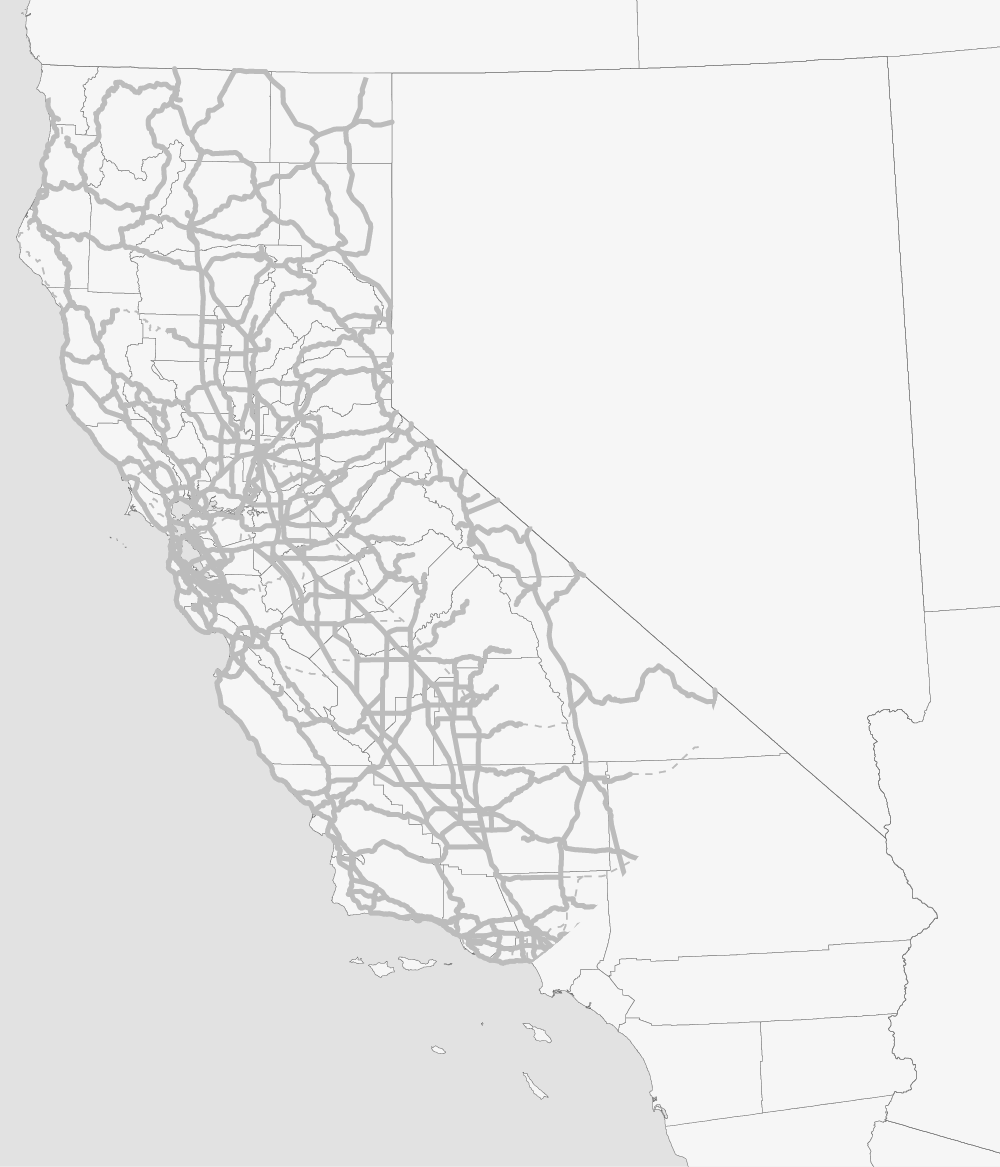
\includegraphics[width=0.7\textwidth]{BFS.png}
    \caption{Breadth First Search}
    \label{fig:bfs}
\end{figure}

\newpage

We see that our BFS search has explored all over the place. It doesn't know the difference between Redding and Santa Barbara. It doesn't recognize one is farther than the other. And frankly, why should it? Why assume one is farther than the other? The beauty in BFS is that it doesn't assume anything: it tries everything.

In real life we rely on mental shortcuts: prior opinions, stereotypes, etc. to make quick judgements without truly investigating. When we look at the map of California, we naturally judge that going North will not get us to Los Angeles quicker, as we rely on the linear distance we observe between the two cities. But this is ultimately no more than a hueristic: it's not certainly true. Perhaps if we go North to Redding we can get on an uncrowded highway and zoom to Los Angeles? Who knows.

Yet on the hand, heuristics can be useful. They can speed up the time it takes to make a judgement. In the case of search, it prevents us from exploring what are likely unfruitful paths. The only concern is our assumption, but if we feel strongly about this assumption perhaps it's worth the risk of missing out on a better opportunity or path.

And so we introduce A*. A* is a very simple algorithm. It is quite frankly no more than a uniform cost search: prioritizing the next successor to consider based on total cost to arrive at that successor. However, we now also consider some hueristic of our invention. The idea is the same for all heuristics: make an assumption to speed up our judgement.

Here is the same search performed with A*, where we prioritize the next successor based on cost as well as its linear distance to Los Angeles.

\begin{figure}[h]
    \centering
    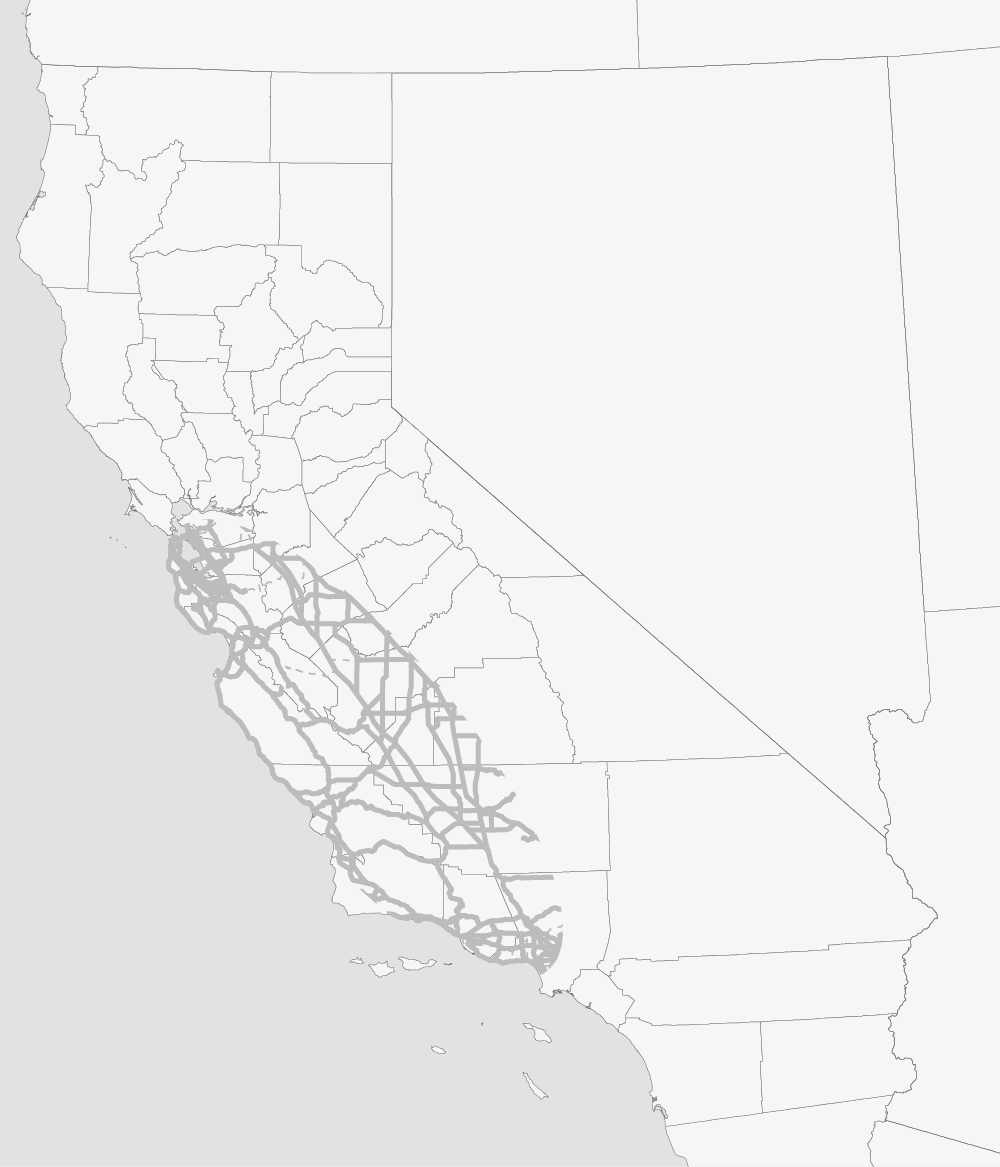
\includegraphics[width=0.7\textwidth]{a-star.png}
    \caption{A* Search With Linear Distance Hueristic}
    \label{fig:a-star}
\end{figure}

\newpage

We explore fewer paths. This algorithm was much easier to run. And in this case, it finds the same correct path as BFS.

\section*{Admissible Hueristics}

But the concern hinted at above is immediately raised: what if our assumption is wrong? What if it turns out there is a faster way to Los Angeles by going North?

In many cases, we just can't be sure. We classify hueristics according to precisely this question. An \textbf{admissible} heuristic is one which will always \textbf{underestimate} the actual cost of the shortest path. If we are certain that we are using an admissable heuristic, we can be certain that our resulting path will always be optimal.

\begin{quote}

\textit{This statement is mathematically provable and an understanding of heuristics is totally dependent upon its comprehension: If we achieve a goal state with a hueristic that, at every node, underestimates the true cost to the goal, then there can be no other unexplored path with a lower total cost than the path found.}

\end{quote}

To understand it we must first understand the uniform cost search. Imagine a uniform cost search on a map. The fringe is quite literally on the ``fringe" of our search: it is its border. Every single point on the fringe is more expensive, in total, than the \textbf{total cost} of the successor we actually explore.

Consider the example above of attempting to find a route from San Francisco to Los Angeles. Suppose the Redding super highway truly exists: suppose it requires us to step just one successor North. Maybe there's a massive cost to make this leap... but if we do we will save time on net. Will our UCS capture this route? Of course it will. At some point, as we traverse further and further South the total cost will eventually outweight this massive cost jump, and we'll attempt it, quickly discovering the highway and finding Los Angeles much quicker. If we never make the jump, that means the \textbf{total cost} of our Southbound route has never even exceeded the cost of the jump.

Now let's add our heuristic. We'll say our heuristic is admissible. Now, our fringe is not only every successor whose total cost exceeds the path we're choosing... it's every successor whose total cost \textbf{and} heuristic value exceeds the path we're choosing. Consider our Redding super highway. We move Southbound constantly. With the added heuristic cost, won't the superhighway never been seen? Not at all. If our hueristic is admissible, this means the estimated cost provided by the heuristic is necessarily lower than the total true cost. Therefore, even if our heuristic is very unfavorable to moving northwards... our algorithm eventually gets to the last node, at which point it must necessarily see the next cost, the cost to get to the goal, as the total true cost. This total true cost cannot exceed the cost of jumping North \textbf{and} our heuristic value, otherwise our heuristic is no longer admissible (assuming the Redding highway is faster).

It is mathematically impossible to obtain a non-optimal solution when running A* with an admissible heuristic.

\subsection*{Obtaining an Admissible Heuristic}

How can we generate a heuristic that is certainly admissible?

The most common method is to ``relax" the constraints of our problem, and estimate the optimal path given these relaxed constraints.

A common example is the map pathing problem. When we choose linear distance, we are quite literally relaxing the constraints—you don't have to follow the road, you can simply drive forward at the maximum speed of your car.

In any case where the constraints are truly relaxed, we necessarily form an admissible heuristic and can be certain that our A* algorithm will produce an optimal result.

\section*{Consistent Heuristics}

In addition to admissibility, heuristics are also graded by \emph{consistency} (also called monotonicity). A heuristic is \emph{consistent} if, for every move from one node to another, the change in the heuristic value does not exceed the actual cost of that move. In other words, the heuristic estimate should decrease by no more than the cost of the step.

For example, if moving east has a cost of 2 and my heuristic decreases from 7 to 3 (a decrease of 4), then the heuristic is \emph{inconsistent} because it decreased by more than the step cost. For consistency, the decrease should be at most 2.

Most admissible heuristics are also consistent. The key benefit to a consistent heuristic is that it avoids visiting the same path twice.

\end{document}

